\chapter{Driven cavity problem}
The driven cavity problem consists in a two-dimensional cavity with an incompressible fluid. The upper wall of the cavity moves at a given velocity, as shown in figure \ref{DrivenCavityImg}. The aim of the problem is to obtain the distribution of velocities inside the cavity.
\begin{figure}
	\centering
	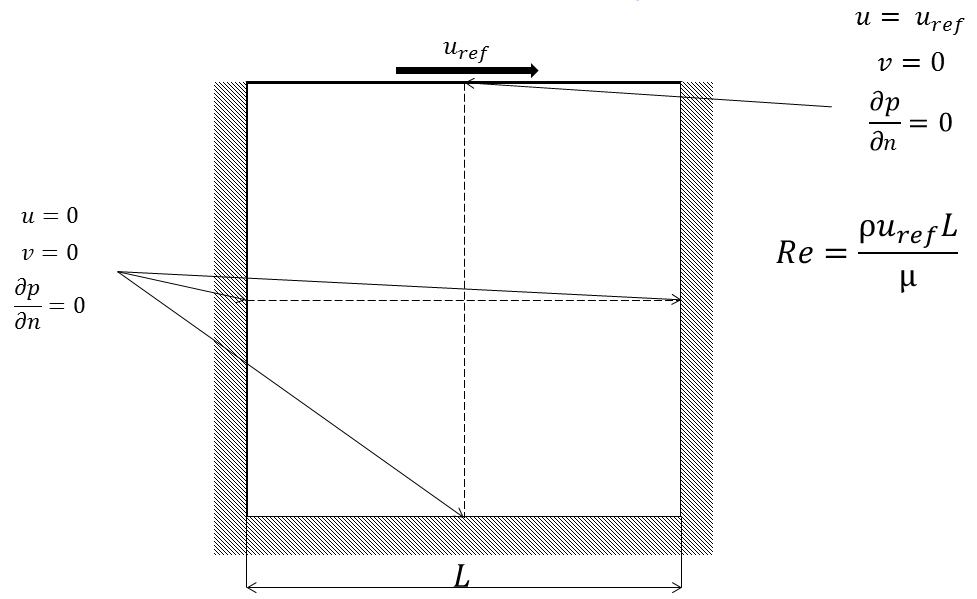
\includegraphics[scale=0.5]{DrivenCavity/DrivenCavity}
	\caption{General scheme of the driven cavity problem}
	\label{DrivenCavityImg}
\end{figure}

\section{Boundary conditions}
It is necessary to impose the conditions defined by figure \ref{DrivenCavityImg}. These boundary conditions modify the discretization coefficients in the boundary nodes.
There are two types of conditions: the prescribed velocity, and the boundary layer conditions. The last ones are defined by assuming that the pressure gradient normal to the wall is 0. For example, in the left wall:
\begin{equation}
	\frac{\partial p}{\partial x}\approx\frac{p_{E}-p_{P}}{\Delta x}=0
\end{equation}
\begin{equation}
P_{P}=p_{E}
\end{equation}
The prescribed velocity is defined using a similar approach. It is assumed that $u_{P}^{n+1}=u^{P}$. To obtain this solution, the pressure gradient has to be equal to zero, so the same expression as in the boundary layer conditions is obtained.
\begin{table}
	\centering
	\begin{tabular}{ |c|c|c|c|c| }
		\hline
		Coefficients & Top & Bottom & Left & Right \\ \hline
		$a_{E}$ & 1 & 0 & 1 & 0 \\ \hline
		$a_{W}$ & 0 & 0 & 0 & 1 \\ \hline
		$a_{N}$ & 0 & 1 & 0 & 0 \\ \hline
		$a_{S}$ & 0 & 0 & 0 & 0 \\ \hline
		$a_{P}$ & 1 & 1 & 1 & 1 \\ \hline
	\end{tabular}
\caption{Discretization coefficients in the boundary}
\end{table}

